\documentclass[t, 				             
			   final,
			   12pt, 				         
			   xcolor={usenames,dvipsnames}, 
			   table]{beamer}

% pacotes utilizados.
\usepackage[alf]{abntex2cite}
\usepackage{amsmath}
\usepackage[brazil]{babel}
\usepackage{booktabs}
\usepackage{caption}
\usepackage{ctable}
\usepackage[utf8]{inputenc}
\usepackage{listings}
\usepackage{multicol}
\usepackage{multirow}
\usepackage{todo}


% configuração do tema
\usetheme[pageofpages=de,
          bullet=square,			
          titleline=true,				
          alternativetitlepage=true,			
          titlepagelogo=imagens/logo-puc,	
          watermarkheight=70px,		
          watermarkheightmult=4	
          ]{Torino}

\setbeamertemplate{sections/subsections in toc}[square]
\setbeamertemplate{bibliography item}[default]

\usecolortheme{freewilly}

% Block Environment
% -------------------------------
\setbeamertemplate {blocks}[default]
\setbeamercolor{block title}{fg=red!0!green!15!blue!85!, bg=red!33!green!37!blue!15!}
\setbeamercolor{block body}{fg=black, bg=red!32!green!33!blue!5}
\setbeamercolor{block title alerted}{fg=white, bg=red!40!black}
\setbeamercolor{block body alerted}{fg=black, bg=red!5!white}
\setbeamercolor{block title example}{fg=white, bg=green!40!black}
\setbeamercolor{block body example}{fg=black, bg=green!5!white}
\setbeamerfont{block title}{size=\scriptsize, series=\bfseries}


\definecolor{javared}{rgb}{0.6,0,0} % for strings
\definecolor{javagreen}{rgb}{0.25,0.5,0.35} % comments
\definecolor{javapurple}{rgb}{0.5,0,0.35} % keywords
\definecolor{javadocblue}{rgb}{0.25,0.35,0.75} % javadoc
 
\lstset{}

\lstdefinestyle{BashInputBasicStyle}{
	language=bash,
	basicstyle=\normalsize\ttfamily,
	columns=fullflexible,
	tabsize=2,
	showstringspaces=false,
	frame=single,
	inputencoding=utf8,
	rulecolor=\color{gray}
}

\lstdefinestyle{BashInputStyle}{
  language=bash,
  basicstyle=\normalsize\ttfamily,
  numbers=left,
  numberstyle=\tiny,
  numbersep=2pt,
  frame=tb,
  columns=fullflexible,
  tabsize=2,
  showstringspaces=false,
  commentstyle=\color{gray},
  inputencoding=utf8,
  rulecolor=\color{gray}
}

\lstdefinestyle{RubyInputStyle}{
    language=ruby,
    basicstyle=\scriptsize\ttfamily,
    keywordstyle=\color{javapurple},
    identifierstyle=\color{black},
    commentstyle=\color{javagreen},
	stringstyle=\color{blue},
    showstringspaces=false,
    numbers=left,
    numberstyle=\color{gray}\tiny,
    tabsize=3,
    extendedchars=\true,
    inputencoding=utf8,
%   frame=single, 
    columns=fixed,
    backgroundcolor=\color{red!32!green!33!blue!5}
}    
%  language=ruby,
%  basicstyle=\normalsize\ttfamily,
%  keywordstyle=\color{OrangeRed},
%  identifierstyle=\color{Turquoise},
%  commentstyle=\color{gray},
%  stringstyle=\color{YellowOrange},
%  numbers=left,
%  numberstyle=\tiny,
%  numbersep=2pt,
%  frame=tb,
%  columns=fullflexible,
%  backgroundcolor=\color{white!80},
%  linewidth=0.9\linewidth,
%  tabsize=2,
%  showstringspaces=false
%  inputencoding=utf8


\lstdefinestyle{JavaInputStyle}{
	language=Java,
	basicstyle=\ttfamily,
	keywordstyle=\color{javapurple}\bfseries,
	stringstyle=\color{javared},
	commentstyle=\color{javagreen},
	morecomment=[s][\color{javadocblue}]{/**}{*/},
	numbers=left,
	numberstyle=\tiny\color{black},
	numbersep=10pt,
	tabsize=2,
	showspaces=false,
	showstringspaces=false,
	frame=tb,
	columns=fullflexible,
	backgroundcolor=\color{white!80},
	linewidth=0.9\linewidth,
	inputencoding=utf8
}

\begin{document}
	\author{Luiz Alberto Ferreira Gomes}
\title{Linguagem Ruby}
\subtitle{Seminários da Computação}
\institute{Curso de Ciência da Computação}
\date{\today}

	\begin{frame}[plain]
  \titlepage
\end{frame}
	\AtBeginSection[]
{
  \begin{frame}{Ruby}
    \tableofcontents[currentsection]
  \end{frame}
}
  
%	\section{Apresentaço do Curso}

%%-------------------------------------------------------------------------------------- Início
\begin{frame}[fragile,t]{Apresentação do Curso}
  \begin{itemize}
    \item Este curso tem como objetivo explorar o \alert{desenvolvimento de aplicações web} considerando 
      \alert{padrões de projetos} fundamentais e filosofias associadas a \alert{arquiteturas modernas} de aplicações web
      , juntamente com os seus principais componentes.
    \item Ao final deste curso, espera-se que o aluno seja capaz de:
    \begin{itemize}
      \item projetar, desenvolver e publicar uma aplicação web;
      \item entender os principais \alert{componentes} da arquitetura web apps e como eles se interagem;
      \item utilizar a plataforma Ruby on Rails;
      \item compreender melhor as \alert{práticas} modernas de engenharia de software.
    \end{itemize}
  \end{itemize}
\end{frame}
%%-------------------------------------------------------------------------------------- Início
\begin{frame}[fragile,t]{Conteúdo Programático}
    \begin{center}
      \begin{tabular}{| p{2cm} | p{8cm} |}
	\hline
	\textbf{Data} & \textbf{Módulo} \\ \hline
	18/09 & Introdução e Conceituação \\ \hline
	25/09 & Ruby on Rails \\ \hline
	02/10 & Interação com Banco de Dados \\ \hline
	09/10 & A Linguagem de Programação Ruby \\ \hline
	16/10 & A Linguagem de Programação Ruby \\ \hline
	23/10 & Middleware \\ \hline
	30/10 & Interface com o Usuário \\ \hline
	\hline
      \end{tabular}
    \end{center}  
\end{frame}
%	\section{Aplicação Web}
%%-------------------------------------------------------------------------------------- Início

%%-------------------------------------------------------------------------------------- Início
\begin{frame}[allowframebreaks, fragile,t]{Aplicação Web}
  \begin{exampleblock}{Definição(Aplicação Web)}
    Uma \alert{aplicação web} é aquela que acessada pelos usuários por meio de uma \alert{rede de computadores}, utiliza
    um \alert{navegador} (em inglês: \textit{browser}); e consiste de uma coleção de \alert{\textit{scripts}} no cliente e 
    no servidor, páginas \alert{HTML} e outros recursos que podem estar espalhados por vários servidores. Ele é 
    acessada pelos usuários via \alert{um endereço} que faz referência a um servidor web (por exemplo: www.inf.pucpcaldadas.br).
  \end{exampleblock}
  
  \begin{itemize}
    \item Exemplos: webmail, lojas virtuais, homebanking, wikis, blogs e etc.
  \end{itemize}
  
\framebreak

  \begin{itemize}
    \item Há um pouco mais do que isso:
    \begin{itemize}
      \item Rede de Computadores:
      \begin{itemize}
        \item a \alert{Internet}, um sistema global de redes de computadores interconectadas.
        \item utiliza o conjunto de protocolos TCP/IP.
      \end{itemize}
      \item Web (World Wide Web):
      \begin{itemize}
	\item um sistema de documentos (em inglês: \textit{web pages}) \alert{vinculados} que são acessados através 
	  da Internet via protocolo HTTP.
	\item Web pages contêm documentos \alert{hypermedia}: textos, gráficos, imagens, vídeos e outros recursos multimídia, juntamente com \textit{hiperlinks} para outras páginas
	\item \alert{Hiperlinks} formam a \alert{estrutura básica} da Web.
	\item A estrutura da Web é a que a torna \alert{útil} e de \alert{valor}.
      \end{itemize}
    \end{itemize}
    \item \underline{Vantagens}:
    \begin{itemize}
      \item \alert{Conveniência} pela utilização um web browser como cliente. 
      \item \alert{Compatibilidade} inerente entre plataformas.
      \item Habilidade de \alert{atualizar} e \alert{manter} as aplicações web sem instalação e distribuição de software
        em vários clientes em potencial.
      \item \alert{Redução} dos custos de TI.
    \end{itemize}
    \item \alert{Desvantagens}:
    \begin{itemize}
      \item Interfaces com usuário ainda \alert{não são tão boas} quanto as das aplicações tradicionais.
      \item Maior risco de \alert{comprometimento} da \alert{privacidade} e \alert{segurança dos dados}.
      \item Mais \alert{difícil} de \alert{desenvolver} e \alert{depurar} do que uma aplicação tradicional, pois 
        existem mais partes a se considerar.
    \end{itemize}
  \end{itemize}
\end{frame}
%%-------------------------------------------------------------------------------------- Início
%	\section{Apresentaço do Curso}

%%-------------------------------------------------------------------------------------- Início
\begin{frame}[fragile,t]{Apresentação do Curso}
  \begin{itemize}
    \item Este curso tem como objetivo explorar o \alert{desenvolvimento de aplicações web} considerando 
      \alert{padrões de projetos} fundamentais e filosofias associadas a \alert{arquiteturas modernas} de aplicações web
      , juntamente com os seus principais componentes.
    \item Ao final deste curso, espera-se que o aluno seja capaz de:
    \begin{itemize}
      \item projetar, desenvolver e publicar uma aplicação web;
      \item entender os principais \alert{componentes} da arquitetura web apps e como eles se interagem;
      \item utilizar a plataforma Ruby on Rails;
      \item compreender melhor as \alert{práticas} modernas de engenharia de software.
    \end{itemize}
  \end{itemize}
\end{frame}
%%-------------------------------------------------------------------------------------- Início
\begin{frame}[fragile,t]{Conteúdo Programático}
    \begin{center}
      \begin{tabular}{| p{2cm} | p{8cm} |}
	\hline
	\textbf{Data} & \textbf{Módulo} \\ \hline
	18/09 & Introdução e Conceituação \\ \hline
	25/09 & Ruby on Rails \\ \hline
	02/10 & Interação com Banco de Dados \\ \hline
	09/10 & A Linguagem de Programação Ruby \\ \hline
	16/10 & A Linguagem de Programação Ruby \\ \hline
	23/10 & Middleware \\ \hline
	30/10 & Interface com o Usuário \\ \hline
	\hline
      \end{tabular}
    \end{center}  
\end{frame}
%%-------------------------------------------------------------------------------------- Início
\begin{frame}[fragile,t]{Histórico}
  \begin{figure}[h!]
    \centering
    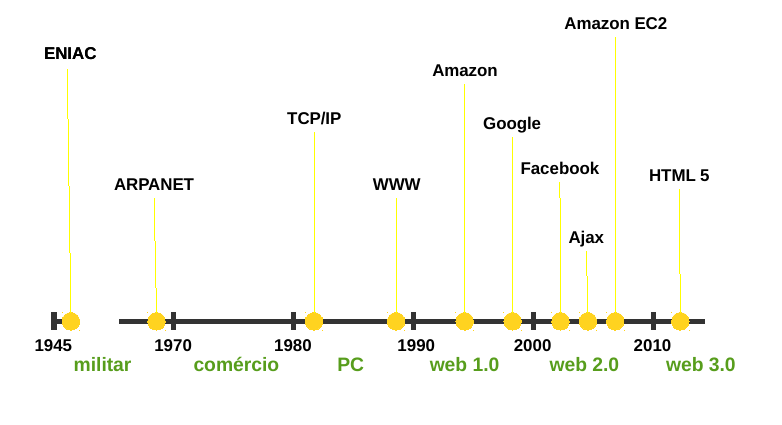
\includegraphics[width=0.95\textwidth]{imagens/historico.png}
  \end{figure} 
\end{frame}
%%-------------------------------------------------------------------------------------- Início
\begin{frame}[fragile,t]{Web 1.0, 2.0 e 3.0}
  \begin{itemize}
    \item \alert{Web 1.0} : páginas estáticas e primeiros modelos de negócios.
    \item \alert{Web 2.0} : interactividade(Ajax), redes sociais e comércio eletrônico.
    \item \alert{Web 3.0} : 'Web Inteligente', interpretação da informação auxiliada por máquina 
    \begin{itemize}
      \item exemplo: sistemas de recomendação.
    \end{itemize}
    \item Base tecnológica da Web 2.0 e 3.0.
    \begin{itemize}
      \item javascript, xml, json(ajax).
      \item interoperabilidade via Web Services.
      \item infraestrutura via modelos de \alert{computação em nuvem} (IAAS, PAAS e SAAS)
      \item aplicações móveis
    \end{itemize}
  \end{itemize}
\end{frame}
%%-------------------------------------------------------------------------------------- Início
\begin{frame}[allowframebreaks, fragile,t]{Modelos de Computação em Nuvem}
  
  \begin{itemize}

    \item \alert{IAAS (Infraestructure As A Service)} : fornece a insfraestrutura computacional
      física ou máquinas virtuais e outros recursos discos, firewalls, endereços IP e etc.
    \begin{itemize}
     \item exemplos: Amazon EC2, Windows Azure, Google Compute Engine.
    \end{itemize}
    
    \item \alert{PAAS (Platform as a Service)} : fornece plataformas computacionais que tipicamente incluem sistemas operacionais,
      ambientes para execução de programas, bancos de dados, servidores web e etc.
    \begin{itemize}
     \item exemplos: AWS Elastic Beanstalk, Windows Azure, Heroku e Google App Engine
    \end{itemize}

    \item \alert{SAAS (Software as a Service)} : fornece acesso sob demanda às aplicações de software, sem que o usuário
      tem que se preocupar com sua instalação, configuração e execução.
    \begin{itemize}
     \item exemplos: Google Apps e Microsoft 365.
    \end{itemize}
 
  \end{itemize}
 
\end{frame}
%	%\section{Arquiteturas de WebApps?}
%%-------------------------------------------------------------------------------------- Início
\begin{frame}[allowframebreaks, fragile,t]{Arquiteturas de Aplicações Web}
  \begin{itemize}
    \item As aplicações \alert{web modernas} envolvem uma quantidade significativa de \alert{complexidade}.
    \begin{itemize}
      \item especialmente no lado do servidor.
    \end{itemize}
    \item Uma típica aplicação web envolve \alert{inúmeros protocolos}, \alert{linguagens de programação} e 
      \alert{tecnologias} que compõem a pilha de tecnologia web. 
    \item Desenvolver, manter e ampliar uma aplicação web complexa é \alert{difícil}.
    \begin{itemize}
      \item mas, construindo-o usando uma \alert{base de princípios de sólidos de projeto} pode-se simplificar 
      cada uma dessas tarefas. 
    \end{itemize}
    \item Engenheiros de software usam \alert{abstrações} para lidar com este tipo de complexidade.
    \begin{itemize}
      \item \textit{Design patterns} fornecem abstrações úteis para sistemas orientados a objetos.
    \end{itemize} 
  \end{itemize}
\end{frame}
%%-------------------------------------------------------------------------------------- Início
\begin{frame}[allowframebreaks, fragile,t]{Design Patterns}
  \begin{exampleblock}{Definição (Design Patterns)}
    Um padrão de projeto é uma descrição da \alert{colaboração de objetos} que interagem para resolver 
    um problema de software em geral dentro de um contexto particular.
  \end{exampleblock}
  \begin{itemize}
    \item Um design pattern é um \alert{modelo abstrato} que pode ser aplicado recorrentemente.
    \item A idéia é aplicar padrões de projeto, a fim de \alert{resolver problemas específicos} que ocorrem 
      durante a construção de sistemas reais.
    \item Os padrões de projeto fornecem uma maneira de \alert{comunicar} as soluções em um projeto, ou seja, 
      é a terminologia que engenheiros de software usam para falar sobre projetos.
  \end{itemize}
\end{frame}
%%-------------------------------------------------------------------------------------- Início
\begin{frame}[allowframebreaks, fragile,t]{Modelo Cliente-Servidor}
	\begin{itemize}
		\item A arquitetura \alert{cliente-servidor} é a arquitetura mais básica para descrever a cooperação
		entre os componentes de uma aplicação web.
		\item A arquitetura cliente-servidor pode ser subdividia em:
		\begin{itemize}
			\item \alert{servidor} que "escuta" por requisições e fornece os serviços ou recursos de acordo com 
			cada  uma.
			\item \alert{cliente} que estabelece a conexão com o servidor para requisitar serviços ou recursos.
		\end{itemize}
		\item Existe um protocolo \alert{request/response} associado com qualquer arquitetura cliente-servidor.
	\end{itemize}
	\begin{figure}[h!]
		\centering
		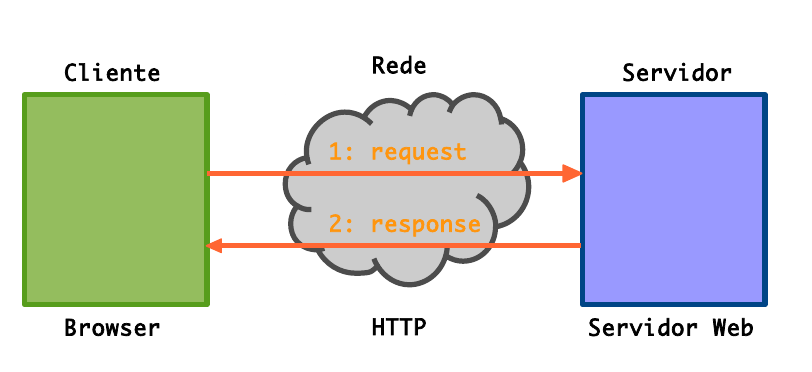
\includegraphics[width=0.90\textwidth]{imagens/cliente-servidor-1.png}
		\caption{Arquitetura cliente servidor.}
	\end{figure} 
	
\framebreak
  \begin{itemize}
    \item É sem dúvida é o padrão de projeto de arquitetura mais conhecido
    \item O ponto chave de uma arquitetura cliente-servidor é \alert{distribuir} os componentes de uma 
      aplicação entre o cliente o servidor de alguma forma. 
    \begin{itemize}
        \item o servidor realiza as tarefas, consultas e transações
        \item o cliente fica com uma responsabilidade menor: a de receber informações
    \end{itemize} 
    \item A fim de construir aplicações web complexas, vários design patterns ajudam a \alert{organizar} como peças 
      são dispostas dentro da arquitetura cliente-servidor.
  \end{itemize}
\end{frame}
%%-------------------------------------------------------------------------------------- Início
\begin{frame}[allowframebreaks, fragile,t]{Arquitetura N-Tier}
  \begin{exampleblock}{Definição (Arquitetura N-Tier)}
    A arquitetura n-tier é um \textit{design pattern} muito útil que estrutura o modelo cliente-servidor.
  \end{exampleblock}
  \begin{itemize}
    \item Este padrão de projeto é baseado no conceito de \alert{quebrar} um sistema em partes diferentes ou 
      camadas que podem ser separados fisicamente:
    \begin{itemize}
      \item cada camada é responsável por fornecer uma \alert{funcionalidade específica} ou coesa. 
      \item uma camada apenas interage com as \alert{camadas adjacentes} a ela por meio de uma 
	\alert{estrutura} bem definida por meio de \alert{interfaces}.
    \end{itemize}
  \end{itemize}
  \begin{exampleblock}{Exemplos (Arquitetura 2-Tier)}
    \begin{itemize}
      \item Servidores de impressão
      \item Aplicações web antigas:
      \begin{itemize}
        \item Interface com o usuário (navegador) residia no cliente (thin). 
        \item Servidor fornecia as páginas estáticas (HTML). 
        \item Interface entre os dois via \textit{Hypertext Transfer Protocol} (HTTP).
      \end{itemize}
    \end{itemize}
  \end{exampleblock}
  \begin{itemize}
    \item Camadas \alert{adicionais} aparecem quando a \alert{funcionalidade} do aplicativo é ainda 
      \alert{mais dividida}.
    \item Quais são as vantagens de um tal projeto? 
    \begin{itemize}
      \item A abstração fornece um meio para \alert{gerenciar} a complexidade. 
      \item Camadas podem ser atualizados ou substituídos de forma \alert{independente} 
	a medida que os requisitos ou tecnologia.
      \begin{itemize}
       \item  a nova só precisa usar as \alert{mesmas interfaces} que a antiga utilizada. 
      \end{itemize}
      \item Ele fornece um \alert{equilíbrio} entre inovação e padronização. 
      \item Sistemas tendem a ser muito mais \alert{fáceis} de construir, manter e atualizar.
    \end{itemize}
  \end{itemize}

\end{frame}
%%-------------------------------------------------------------------------------------- Início
\begin{frame}[allowframebreaks, fragile,t]{Arquitetura 3-Tiers}
  \begin{itemize}
    \item Uma das mais comuns é a arquitetura em 3 camadas: 
    \begin{itemize}
      \item Apresentação
      \begin{itemize}
       \item a interface com o usuário. 
      \end{itemize}     
      \item Aplicação (lógica)
      \begin{itemize}
	\item recupera modifica e$/$ou exclui dados na camada de dados, e envia os resultados do processamento
	para a camada de apresentação. 
      \end{itemize}
      \item Camada de dados
      \begin{itemize}
       \item a fonte dos dados associados ao aplicativo.
      \end{itemize}
    \end{itemize}
 
    \item As aplicações web modernas frequentemente são construídas \alert{utilizando} uma arquitetura em 3 camadas: 
    \begin{itemize}
      \item Apresentação
      \begin{itemize}
	\item o navegador web do usuário. 
      \end{itemize}

      \item Aplicação (lógica) 
      \begin{itemize}     
	\item o servidor web e lógica associada com \alert{geração} de conteúdo web dinâmico.
	\item por exemplo, a coleta e formatação do resultados de uma pesquisa. 
      \end{itemize}
      
      \item Camada de dados
      \begin{itemize}    
	\item um banco de dados.
      \end{itemize}
      
    \end{itemize}
    
  \end{itemize}
\end{frame}
%%-------------------------------------------------------------------------------------- Início
%\begin{frame}[allowframebreaks, fragile,t]{Arquitetura 6-Tiers para Aplicações Web }
%  \begin{itemize}
%    \item A camada de aplicação é frequentemente subdividida em dois níveis:
%    \begin{itemize} 
%      \item Camada de lógica de negócios
%      \begin{itemize}
%	\item modelos os \alert{objetos de negócios} associados ao aplicativo, por exemplo, contas, estoques, etc.
%	\item captura as regras de negócio associadas a esses objetos.     
%       \end{itemize}      
%      \item Camada de acesso a dados
%      \begin{itemize}
%	\item responsável por acessar os dados e passá-los para a camada de lógica de negócios.
%	\item por exemplo, saldos de contas, transações, etc.
%      \end{itemize}
%    \end{itemize}
%    \item A camada de apresentação é muitas vezes subdividida em dois níveis: 
%    \begin{itemize}
%      \item Camada de clientes
%      \begin{itemize}
%	\item os componentes da interface do usuário do lado do cliente.
%      \end{itemize}
%      
%      \item Apresentação camada de lógica
%      \begin{itemize}
%       \item scripts do lado do servidor para a geração de páginas web. 
%      \end{itemize}
%
%    \end{itemize}
%    \item Finalmente, o servidor web é muitas vezes separados em sua própria camada da Web e o
%    servidor de banco de dados na sua camada de dados.
%  \end{itemize}
%  
%  \begin{figure}[h!]
%    \centering
%    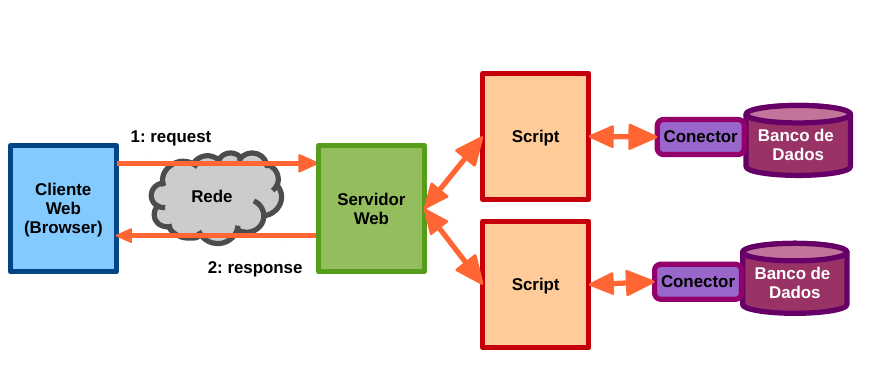
\includegraphics[width=0.95\textwidth]{imagens/cliente-servidor-2.png}
%    \caption{Arquitetura em 6 Camadas.}
%  \end{figure}
%  
%\end{frame}
%%%-------------------------------------------------------------------------------------- Início
	
	\section{Introdução}	
	%-------------------------------------------------------------------------------------- Início
\begin{frame}[fragile,t]{Ruby}
  \begin{itemize}
    \item Linguagem inventada por Yukihiro "Matz" Matsumoto
    \item Versão 1.0 liberada em 1996(Japão)
    \item Popularizado no início de 2005 pelo Rails
  \end{itemize}   
  \begin{figure}[hbt]
    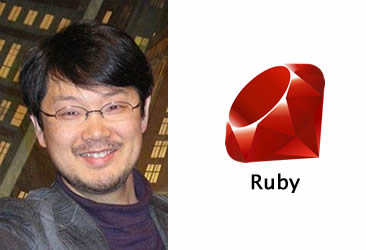
\includegraphics[scale=.5]{imagens/matz.jpg}
  \end{figure}
\end{frame}
%-------------------------------------------------------------------------------------- Início
\begin{frame}[fragile,t]{Ruby}
  \begin{itemize}
    \item Linguagem \alert{dinâmica} e \alert{orientada a objetos}
    \item Elegante, \alert{expressiva} e declarativa
    \item Influenciada pelo Perl, Smalltalk, Eiffel e Lisp
  \end{itemize}   
\end{frame}
%-------------------------------------------------------------------------------------- Início
\begin{frame}[fragile,t]{..Java..}
  \begin{lstlisting}[style=JavaInputStyle]
    public class Print3Times {
      public static void main(String[] args) {
        for(int i = 0; i < 3; i++) {
          System.out.println("Hello World!")
        }
      }
    }
  \end{lstlisting}
\end{frame}
%-------------------------------------------------------------------------------------- Início
\begin{frame}[fragile,t]{..Ruby..}
		\lstinputlisting[style=RubyInputStyle, caption=hello.rb]{codigos/ruby/01-ruby-introducao/hello.rb}
\end{frame}
%-------------------------------------------------------------------------------------- Início
\begin{frame}[fragile,t]{Básico do Ruby}
  \begin{itemize}
    \item Indentação de 2 espaços para cada nível aninhado (\alert{recomendado})
    \item \# é utilizado para comentários
    \begin{itemize}
    	\item use com moderação, o código deve ser auto documentado
    \end{itemize}
    \item Scripts utilizam a extensão \verb!.rb! 
		\lstinputlisting[style=RubyInputStyle, caption=hello.rb]{codigos/ruby/01-ruby-introducao/hello.rb}
  \end{itemize}   
\end{frame}
%-------------------------------------------------------------------------------------- Início
\begin{frame}[fragile,t]{Saída na Tela}
  \begin{itemize}
    \item \verb!puts! é método \alert{padrão} para impressão em tela 
    \begin{itemize}
    	\item insere uma quebra de linha após a impressão
    	\item similar ao \verb!System.out.println! do Java
    \end{itemize}
    \item \alert{p} é utilizado para depuração
  \end{itemize}   
\end{frame}
%-------------------------------------------------------------------------------------- Início
\begin{frame}[fragile,t]{Entrada pelo Teclado}
  \begin{itemize}
    \item \verb!gets! é método padrão para receber um valor pelo teclado 
		\begin{lstlisting}[style=RubyInputStyle]
# recebe um valor do tipo string.
nome = gets
  	\end{lstlisting}
    \item Utilize \verb!gets.chomp! para remover o caracter de nova linha.
		\begin{lstlisting}[style=RubyInputStyle]
# remove o caracter de nova linha.
nome = gets.chomp
  	\end{lstlisting}
  	\item Utilize \verb!gets.chomp.to_i! para converter o valor lido para inteiro. 
		\begin{lstlisting}[style=RubyInputStyle]
# converte a string recebida para inteiro.
nome = gets.chomp.to_i
  	\end{lstlisting}
  \end{itemize}   
\end{frame}
%-------------------------------------------------------------------------------------- Início
\begin{frame}[fragile,t]{Convenção de Nomes}
  \begin{itemize}
    \item Variáveis e Métodos
    \begin{itemize}
    	\item em minúsculas e \verb!separada_por_sublinhado! (tenha mais de uma palavra)
    	\item métodos ainda permitem no final os caracteres \verb|?!|
    \end{itemize}
    \item Constantes
    \begin{itemize}
    	\item tanto \verb!TODAS_AS_LETRAS_EM_MAIUSCULAS! ou no formato \verb!CamelCase!
    \end{itemize}
    \item Classes(e módulos)
    \begin{itemize}
    	\item formato \verb!CamelCase! 
    \end{itemize}
  \end{itemize}
\end{frame}
%-------------------------------------------------------------------------------------- Início
\begin{frame}[fragile,t]{Remoção do Ponto-e-Vírgula}
  \begin{itemize}
    \item Não coloque o ponto-e-vírgula no final da linha
    \item Pode ser utilizado para colocar várias declarações em uma linha
    \begin{itemize}
      \item altamente desencorajado
    \end{itemize}
    \begin{lstlisting}[style=RubyInputStyle]
a = 3	
a = 3; b = 5 
    \end{lstlisting}
  \end{itemize}
\end{frame}
%-------------------------------------------------------------------------------------- Início
\begin{frame}[allowframebreaks, fragile,t]{Interactive Ruby (IRB)}
  \begin{itemize}
    \item Console \alert{interativa} para interpretação de comandos Ruby
    \item Instalado com o interpretador Ruby
    \item Permite a \alert{execução} de comandos rapidamente
  \end{itemize}
  \begin{figure}[hbt]
    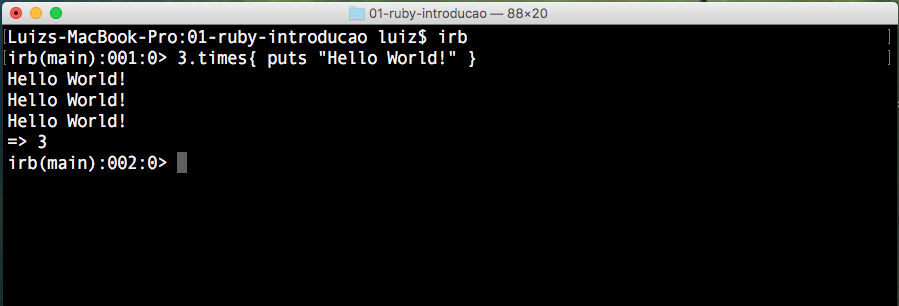
\includegraphics[scale=.35]{imagens/ruby-irb.png}
  \end{figure}
\framebreak
  \begin{itemize}
  	\item Permite a \alert{execução} de \alert{scripts} contendo vários comandos
  \end{itemize}
  \begin{figure}[hbt]
    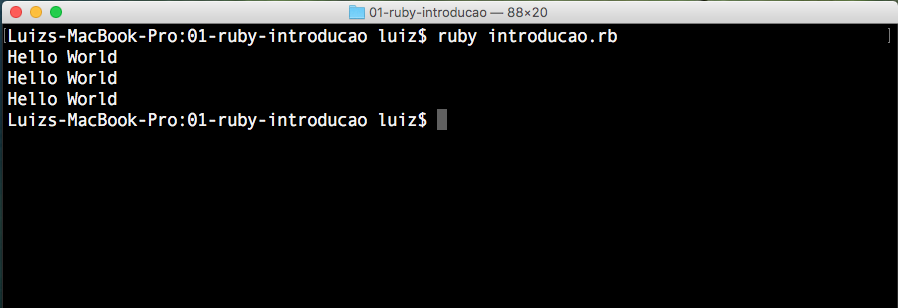
\includegraphics[scale=.35]{imagens/ruby-interpretador.png}
  \end{figure}
\end{frame}
%-------------------------------------------------------------------------------------- Início
\begin{frame}[allowframebreaks,fragile,t]{Exercícios}
  \begin{itemize}
    \item Escreva um script Ruby para imprimir um nome lido teclado 5 vezes.
  \end{itemize}
\framebreak
  \begin{itemize}
    \item \textbf{Solução}:
  \end{itemize}	
  \begin{lstlisting}[style=RubyInputStyle]
nome = gets.chomp
5.times { puts nome }
  \end{lstlisting}
\end{frame}

	\section{Controle de Fluxo}
	%-------------------------------------------------------------------------------------- Início
\begin{frame}[allowframebreaks, fragile,c]{Controle de Fluxo}
  \begin{center}
    \Large \verb!if ... elsif ... else! \\ \verb!case! \\ \verb!unless!
  \end{center}   
\framebreak
  \begin{itemize}
    \item \alert{Não} existe a necessidade de uso de \alert{parênteses} ou \alert{chaves}
    \item \alert{Utilize} a instrução \verb!end! no final do bloco
  \end{itemize}   
  \begin{columns}
    \begin{column}{0.5\textwidth}
    		\lstinputlisting[style=RubyInputStyle, caption=if.rb]{codigos/ruby/02-fluxo-de-controle/if.rb}  
    \end{column}
    \begin{column}{0.5\textwidth}
    		\lstinputlisting[style=RubyInputStyle, caption=unless.rb]{codigos/ruby/02-fluxo-de-controle/unless.rb}  
    \end{column}
  \end{columns}
\framebreak
    		\lstinputlisting[style=RubyInputStyle, caption=case\_1.rb]{codigos/ruby/02-fluxo-de-controle/case_1.rb}  
\framebreak
    		\lstinputlisting[style=RubyInputStyle, caption=case\_2.rb]{codigos/ruby/02-fluxo-de-controle/case_2.rb}  
\end{frame}
%-------------------------------------------------------------------------------------- Início
\begin{frame}[fragile,t]{Operadores Lógicos (em ordem de precedência)}
	\begin{table}[tp] 	
		\setlength{\tabcolsep}{8pt}
    \setlength{\extrarowheight}{2pt}    
		\begin{tabular}{p{2.5cm}l}
    	\toprule
      $<=, <, >, >=$ &  Comparação\\
      $==, !=$ & Igual ou diferente  \\
      $\&\&$ &  Conectivo \textbf{e} \\
      $||$ & Conectivo \textbf{ou} \\
	    \bottomrule
		\end{tabular}
	\end{table}   
\end{frame}
%-------------------------------------------------------------------------------------- Início
\begin{frame}[fragile,t]{True e False}
  \begin{itemize}
    \item \alert{false} e \alert{nil} são booleanos \alert{FALSOS}
    \item Todo o restante é \alert{VERDADEIRO}
	\lstinputlisting[style=RubyInputStyle, caption=true\_false.rb]{codigos/ruby/02-fluxo-de-controle/true_false.rb}
  \end{itemize}   
\end{frame}
%-------------------------------------------------------------------------------------- Início
\begin{frame}[fragile,t]{Exercícios}
  \begin{enumerate}
    \item Digite as seguintes expressões no IRB e verifique os resultados.
  \end{enumerate}
	\begin{lstlisting}[style=RubyInputStyle]
		(32 * 4) >= 129
		false != !true
		true == 4
		false == (847 == '847')
		(!true || (!(100 / 5) == 20) || ((328 / 4) == 82) || false 
	\end{lstlisting}
\end{frame}
%-------------------------------------------------------------------------------------- Início
\begin{frame}[fragile,t]{Recapitulando}
  \begin{itemize}
    \item Existe muitas opções de fluxo de controle
    \item A formato em um linha é muito expressiva
    \item Exceto \verb!nil! e \verb!false!, os demais valores são verdadeiros.
  \end{itemize}
\end{frame}




	\section{Loops e Interações}	
	
\begin{frame}[allowframebreaks, fragile,t]{Loops e Interações}
  \begin{center}
    \Large \verb!loop! \\ \verb!while e until! \\ \verb!for! \\ \verb!each e times!
  \end{center}   
\framebreak

  \begin{itemize}
	\item \verb!loop!
  \end{itemize}
  \lstinputlisting[style=RubyInputStyle, caption=loop.rb]{codigos/ruby/03-loop-e-interacoes/loop.rb}

\framebreak
  \begin{itemize}
	\item \verb!while e until!
  \end{itemize}
     
  \begin{columns}
    \begin{column}{0.5\textwidth}
  \lstinputlisting[style=RubyInputStyle, caption=while.rb]{codigos/ruby/03-loop-e-interacoes/while.rb}
    \end{column}
    \begin{column}{0.5\textwidth}  %%<--- here
  \lstinputlisting[style=RubyInputStyle, caption=until.rb]{codigos/ruby/03-loop-e-interacoes/until.rb}
    \end{column}
  \end{columns}

\framebreak
  \begin{itemize}
		\item \verb!for! (\alert{dificilmente empregado})
    \item \verb!each/times! é preferível
  \end{itemize}
  
  \lstinputlisting[style=RubyInputStyle, caption=for\_loop.rb]{codigos/ruby/03-loop-e-interacoes/for_loop.rb}

\framebreak
  \begin{itemize}
	\item \verb!each!
  \end{itemize}
     
  \begin{columns}
    \begin{column}{0.5\textwidth}
  \lstinputlisting[style=RubyInputStyle, caption=each\_1.rb]{codigos/ruby/03-loop-e-interacoes/each_1.rb}  
    \end{column}
    \begin{column}{0.5\textwidth} 
  \lstinputlisting[style=RubyInputStyle, caption=each\_2.rb]{codigos/ruby/03-loop-e-interacoes/each_2.rb}

    \end{column}
  \end{columns}
\end{frame}
\begin{frame}[allowframebreaks,fragile,t]{Hora de Colocar as Mão na Massa}
  \begin{enumerate}
    \item Escreva um \textit{script} Ruby leia o nome de um jogador do jogo de adivinha e 
      apresente o valor lido.
    \item O \textit{script} Ruby deverá sortear um número de 1 a 10 e permite que 
    o usuário tente 3 vezes até acertá-lo. A cada tentativa errada, o programa informa
    se o número a adivinhar está abaixo ou acima. \textbf{Dica:} utilize rand(n) + 1 
  \end{enumerate}
  \framebreak
\end{frame}
%-------------------------------------------------------------------------------------- Início
\begin{frame}[allowframebreaks,fragile,t]{Solução do Exercício}
  \lstinputlisting[style=RubyInputStyle, caption=loop.rb]{codigos/ruby/03-loop-e-interacoes/jogo-de-adivinha.rb}
\end{frame}

\begin{frame}[fragile,t]{Recapitulando}
  \begin{itemize}
    \item Existe muitas opções de loops e interações
    \item \verb!each! é \alert{preferível} ao loop \verb!for! para percorrer arrays
  \end{itemize}
\end{frame}




	\section{Funções e Métodos}
	
\begin{frame}[fragile,t]{Funções e Métodos}
  \begin{itemize}
    \item Tecnicamente, uma \alert{função} é definida \alert{fora} de uma classe
    \item Um \alert{método} é definido dentro de uma classe
    \item Em Ruby, \alert{toda} função/método é pertence a pelo menos uma classe
    \begin{itemize}
      \item nem sempre explicitamente escrito em uma classe
    \end{itemize}
  \end{itemize}
  \framebreak   
  \begin{center}
    Conclusão: Toda \alert{função} é na verdade um \alert{método} em Ruby  
  \end{center}
\end{frame}

\begin{frame}[fragile,t]{Métodos}
  \begin{itemize}
    \item Parênteses são \alert{opcionais}
    \begin{itemize}
      \item tanto para definição quanto para a chamada do método
    \end{itemize}
    \item Usado para tornar o código mais claro
  \end{itemize}
  \begin{block}{parens.rb}
  	\lstinputlisting[style=RubyInputStyle]{codigos/ruby/04-funcoes-e-metodos/parens.rb}
  \end{block}
  
    
\end{frame}

\begin{frame}[fragile,t]{Parâmetros e Retorno}
  \begin{itemize}
    \item Não é necessário declarar o tipo dos parâmetros
    \item O método pode retornar qualquer valor
    \item O comando \verb!return! é opcional
    \begin{itemize}
      \item o valor da \alert{última linha} executada é retornada 
    \end{itemize}
  \end{itemize}
  
  \lstinputlisting[style=RubyInputStyle, caption=return\_optional.rb]{codigos/ruby/04-funcoes-e-metodos/return_optional.rb}
    
\end{frame}

\begin{frame}[fragile,t]{Nomes de Métodos Expressivos}
  \begin{itemize}
    \item Nomes de métodos podem terminar com:
    \begin{itemize}
    	\item \alert{'?'} - métodos com retorno booleano
    	\item \alert{'!'} - métodos com efeitos colaterais
    \end{itemize}
    
	\lstinputlisting[style=RubyInputStyle, caption=expressive.rb]{codigos/ruby/04-funcoes-e-metodos/expressive.rb}
  \end{itemize}   
\end{frame}

\begin{frame}[fragile,t]{Argumentos Padrões(Defaults)}
  \begin{itemize}
    \item Métodos podem ter argumentos padrões
    \begin{itemize}
    	\item se o valor é passado, ele é utilizado
    	\item senão, o valor padrão é utilizado
    \end{itemize}
  \end{itemize}  
  \lstinputlisting[style=RubyInputStyle, caption=default\_args.rb]{codigos/ruby/04-funcoes-e-metodos/default_args.rb}
\end{frame}

\begin{frame}[fragile,t]{Quantidade Variável de Argumentos}
  \begin{itemize}
    \item \alert{*} prefixa o parâmetro com quantidade variável de argumentos
  \end{itemize}
  \begin{itemize}
    \item Pode ser utilizado com parâmetros no início, meio e final
  \end{itemize}
  \lstinputlisting[style=RubyInputStyle, caption=splat.rb]{codigos/ruby/04-funcoes-e-metodos/splat.rb}
\end{frame}
%-------------------------------------------------------------------------------------- Início
\begin{frame}[fragile,t]{Exercícios}
  \begin{enumerate}
    \item Escreva uma função que receba como parâmetro um custo retorna a taxa de entrega
		de acordo com a seguinte regra:
		\begin{itemize}
			\item a taxa de entrega será igual a 10.00 se o custo for menor do que 25.00;
			\item a taxa será igual a 20.00 se o custo for menor do que 100.00;
			\item a taxa a taxa será igual a 30.00 se o custo for menor do que 200.00;
			\item a taxa será igual a 35.00 se o custo for maior ou igual do que 200.00;
		\end{itemize} 
  \end{enumerate}
\end{frame}

\begin{frame}[fragile,t]{Recapitulando}
  \begin{itemize}
    \item \alert{Não há necessidade} de declarar o tipo de parâmetro passado ou retornado (linguagem dinâmica)
    \item \verb!return! é \alert{opcional} - a última linha executável é "retornada"
    \item Permite métodos com \alert{quantidade variável} de argumentos ou argumentos padrão
  \end{itemize}
\end{frame}




	\section{Blocos}	
	
\begin{frame}[allowframebreaks, fragile,t]{Blocos}
  \begin{itemize}
    \item "Pedaço" de código
    \begin{itemize}
      \item escrito entre chaves(\{\}) ou entre \alert{do} e \alert{end}
      \item passado para métodos como o \alert{último} parâmetro
    \end{itemize}
    \item \textbf{Convenção} 
    \begin{itemize}
      \item use chaves(\{\}) quanto o bloco contém uma linha
      \item use \alert{do} e \alert{end} quando o bloco contém múltiplas linhas
    \end{itemize}
    \item Frequentemente utilizado em \alert{iteração}
  \end{itemize}
  
  \lstinputlisting[style=RubyInputStyle, caption=times.rb]{codigos/ruby/04-blocos/times.rb}
    
\end{frame}

\begin{frame}[fragile,t]{Utilizando Blocos}
  \begin{itemize}
    \item Duas técnicas para utilizar blocos nos métodos
    \item \textbf{Implicitamente:}
    \begin{itemize}
      \item use \verb!block_given?! para checar se o bloco foi passado
      \item use \verb!yield! para \alert{chamar} o bloco
    \end{itemize}
    \item \textbf{Explicitamente:}
    \begin{itemize}
      \item use \verb!&?! como prefixo do último parâmetro
      \item use \verb!call! para \alert{chamar} o bloco
    \end{itemize} 
  \end{itemize}   
\end{frame}

\begin{frame}[fragile,t]{Técnica Implícita}
  \begin{itemize}
    \item Necessário checar com \verb!block_given?! 
    \begin{itemize}
    	\item se não uma excessão será lançada
    \end{itemize}
    
	\lstinputlisting[style=RubyInputStyle, caption=implicit\_blocks.rb]{codigos/ruby/04-blocos/implicit_blocks.rb}
  \end{itemize}   
\end{frame}

\begin{frame}[fragile,t]{Técnica Explícita}
  \begin{itemize}
    \item Necessário checar com \verb!nil?! 
    
	\lstinputlisting[style=RubyInputStyle, caption=implicit\_blocks.rb]{codigos/ruby/04-blocos/explicit_blocks.rb}
  \end{itemize}   
\end{frame}

\begin{frame}[fragile,t]{Recapitulando}
  \begin{itemize}
    \item Blocos são apenas \alert{trechos} de códigos que podem ser passados para métodos
    \item Tanto explicitamente quanto implicitamente
  \end{itemize}
\end{frame}




	\section{Strings}	
	
\begin{frame}[allowframebreaks, fragile,t]{Strings}
  \begin{itemize}
    \item Strings com aspas simples
    \begin{itemize}
      \item permitem a utilização de \alert{'} com $\backslash$
      \item mostra a string como foi escrita 
    \end{itemize}
    \item Strings com aspas duplas 
    \begin{itemize}
      \item interpreta caracteres especiais como $\backslash$n e $\backslash$t
      \item permite a interpolação de strings, evitando concatenação
    \end{itemize}
  \end{itemize}
  
  \lstinputlisting[style=RubyInputStyle, caption=strings.rb]{codigos/ruby/06-strings/strings.rb}
\pagebreak
  \begin{itemize}
    \item Métodos terminados com \alert{!} modificam a string
    \begin{itemize}
      \item a maioria retorna apenas um novo string
    \end{itemize}
    \item Permite o uso do \%Q\{textos longos com multiplas linhas\}
    \begin{itemize}
      \item o mesmo comportamento de strings com aspas duplas
    \end{itemize} 
    \item \alert{É essencial dominar a API de Strings do Ruby}
  \end{itemize}  
  
  \lstinputlisting[style=RubyInputStyle, caption=more\_strings.rb]{codigos/ruby/06-strings/more_strings.rb} 
\end{frame}

\begin{frame}[fragile,t]{Símbolos}
  \begin{itemize}
    \item \alert{:simbolo} $-$ string altamente otimizadas
    \begin{itemize}
      \item ex. :domingo, :dolar, :calcio, :id
    \end{itemize}
    \item Constantes que não precisam ser pré-declaradas
    \item Garantia de \alert{unicidade} e \alert{imutabilidade}
    \item Podem ser convertidos para uma \alert{String} com \alert{to\_s} 
    \begin{itemize}
      \item ou de \alert{String} para \alert{Símbolo} com \alert{to\_sym}
    \end{itemize}
  \end{itemize}   
\end{frame}
%-------------------------------------------------------------------------------------- Início
% \begin{frame}[allowframebreaks, fragile,t]{Exercícios}
%  \begin{enumerate}
%    \item Escreva os \textit{script} em Ruby e verifique os resultados após a sua execução.
%  \end{enumerate}
%	  \lstinputlisting[style=RubyInputStyle, caption=more\_strings.rb]{codigos/ruby/06-strings/more_strings.rb} 
%\end{frame}

\begin{frame}[fragile,t]{Recapitulando}
  \begin{itemize}
    \item A interpolação evita a concatenação de strings
    \item Strings oferecem uma API muito útil
  \end{itemize}
\end{frame}

\begin{frame}[allowframebreaks, fragile,t]{Exercícios}
  \begin{enumerate}
    \item Refatore o jogo de adivinhar nos seguintes métodos:
    \begin{itemize}
      \item {\bf da\_boas\_vindas} que dá boas vindas e retorna o nome do usuário.
      \item {\bf sorteia\_numero\_screto} que retorna o número secreto sorteado.
      \item {\bf pede\_um\_numero} retorna o numero digitado pelo usuário.
      \item {\bf verifica\_se\_acertou } retorna um booleano se o usuário acertou ou não o número secreto.
      \item {\bf nao\_quer\_jogar} retorna se o usuário apos as tentativas quer jogar outra vez ou não.
      \item {\bf joga } método que joga as três tentativas chamando os métodos necessários.
    \end{itemize}
  \end{enumerate}
%  \lstinputlisting[style=RubyInputStyle, caption=splat.rb]{codigos/ruby/04-funcoes-e-metodos/jogo-de-adivinha.rb}
\end{frame}





	\section{Arrays}	
	
\begin{frame}[allowframebreaks, fragile,t]{Arrays}
  \begin{itemize}
    \item Coleção de objetos (auto-expandível)
    \item Indexado pelo operador (método) \alert{[ ]}
    \item Pode ser indexado por números negativos ou intervalos
    \item Tipos heterogêneos são permitidos em um mesmo array
    \item \%\{str1 str2\} pode ser utilizado para criar um array de strings
  \end{itemize}
  
  \lstinputlisting[style=RubyInputStyle, caption=arrays.rb]{codigos/ruby/07-arrays/arrays.rb}
\pagebreak
  \begin{itemize}
    \item Modificando arrays:
    \begin{itemize}
      \item criação: \alert{= [ ]}
      \item inclusão: \alert{push} ou {<<}
      \item remoção: \alert{pop} ou {shift}
    \end{itemize}
    \item Extração randômica de elementos com \alert{sample}
    \item Classificação ou inversão com \alert{sort!} ou {reverse!}
  \end{itemize}  
  
  \lstinputlisting[style=RubyInputStyle, caption=arrays2]{codigos/ruby/07-arrays/arrays2.rb}
  
\pagebreak
  \begin{itemize}
    \item Métodos úteis
    \begin{itemize}
      \item \alert{each} - percorre um array
      \item \alert{select} - filtra por seleção
      \item \alert{reject} - filtra por rejeição
      \item \alert{map} - modifica cada elemento do array
    \end{itemize}
  \end{itemize}  
  
  \lstinputlisting[style=RubyInputStyle, caption=arrays2]{codigos/ruby/07-arrays/array_processing.rb}

\end{frame}
%-------------------------------------------------------------------------------------- Início
\begin{frame}[allowframebreaks,fragile,t]{Exercícios}
  \begin{enumerate}
    \item Escreva um \textit{script} em Ruby que receba pelo teclado um array de tamanho 5 e um número e retorne a mensagem "o número está no array" ou "o número não está no array".  A verificação deverá ser feita por um método.
  \end{enumerate}
\end{frame}

\begin{frame}[fragile,t]{Recapitulando}
  \begin{itemize}
    \item A API de arrays é flexível e poderosa
    \item Existem diversas formas de processar um elemento do array
  \end{itemize}
\end{frame}




	\section{Hashes}	
	
\begin{frame}[allowframebreaks, fragile,t]{Hashes}
  \begin{itemize}
    \item \alert{Coleção indexada} de objetos
    \item Criados com \{\} ou \alert{Hash.new}
    \item Também conhecidos como \alert{arrays associativos}
    \item Pode ser indexado com \alert{qualquer} tipo de dados
    \begin{itemize}
      \item não apenas com \alert{inteiros}
    \end{itemize}
    \item Acessados utilizando o operador \alert{[ ]}
    \item Atribuição de valores poder feita usando:
    \begin{itemize}
      \item \alert{$=>$} (criação)
      \item \alert{$[  ]$} (pós-criação)
    \end{itemize}
  \end{itemize}
  
  \lstinputlisting[style=RubyInputStyle, caption=hashes.rb]{codigos/ruby/09-hashes/hashes.rb}
\pagebreak
  \begin{itemize}
    \item E se tentarmos \alert{acessar} um valor em Hash que \alert{não existe}?
    \begin{itemize}
      \item \alert{nil} é retornado
    \end{itemize}
    \item Se o Hash é criado com \alert{Hash.new(0)} 0 é retornado.
  \end{itemize}  
  
  \lstinputlisting[style=RubyInputStyle, caption=word\_frequency.rb]{codigos/ruby/09-hashes/word_frequency.rb}
  
\pagebreak
  \begin{itemize}
    \item A partir da versão 1.9
    \begin{itemize}
      \item A ordem de criação do Hash é \alert{mantida}
      \item A sintaxe \alert{simbolo:} pode ser utilizada, se símbolos são utilizados como chave
      \item Se o Hash é o \alert{último argumento}, \{\} são opcionais
    \end{itemize}
  \end{itemize}  
  
  \lstinputlisting[style=RubyInputStyle, caption=more\_hashes.rb]{codigos/ruby/09-hashes/more_hashes.rb}

\end{frame}

%-------------------------------------------------------------------------------------- Início
%\begin{frame}[fragile,t]{Exercícios}
%  \begin{enumerate}
%    \item Escreva os \textit{script} em Ruby e verifique os resultados após a sua execução.
%  \end{enumerate}
%	\begin{lstlisting}[style=RubyInputStyle]
%opostos = {positivo: "negativo"
%, aberto: "fechado"
%, direita: "esquerda"}
%opostos.each_key { |key| puts key }
%opostos.each_value { |value| puts value }
%opostos.each { |key, value| puts "O oposto de #{key} eh #{value}" } 
%	\end{lstlisting}
%\end{frame}

\begin{frame}[fragile,t]{Recapitulando}
  \begin{itemize}
    \item Hashes são \alert{coleções indexadas}
    \item Usado de forma \alert{similar aos arrays}
  \end{itemize}
\end{frame}

\begin{frame}[allowframebreaks, fragile, t]{Hora de Colocar as Mãos na Massa}
  \begin{enumerate}
    \item Modifique o jogo de adivinhação para permitir que o sistema me informe, antes de  uma jogada, 
		os números que já foram chutados e me impeça o usuário de digitar um número repetido.

    \item Modifique o jogo de adivinhação para permitir que o usuário escolha o nível de dificuldade 
		que poderá variar de 1 (fácil) a 5 (difícil). A faixa de números aleatórios que o sistema 
		gerará variará de acordo com o nível: 1(1-30), 2(1-60), 3(1-100), 4(1-150) e 5(1-200).
    
  \end{enumerate}
\end{frame}




	\section{Classes e Objetos}	
	
\begin{frame}[fragile,t]{OO}
  \begin{itemize}
    \item OO possibilita identificar "coisas" que serão tratadas pelo programa
    \item \alert{Classes} são descrições dessas \alert{"coisas"} e container de métodos
    \item Objetos são \alert{instâncias} dessas classes
    \item Objetos contêm \alert{variáveis de instância} (estado)
  \end{itemize}
\end{frame}

\begin{frame}[fragile,t]{Variáveis de Instância}  
 \begin{itemize}
    \item Iniciam com: \alert{@}
    \begin{itemize}
      \item exemplo: @nome
    \end{itemize}
    \item Não há necessidade de declará-las 
    \item Disponível para todas as instâncias dos métodos da classe
  \end{itemize}
\end{frame}

\begin{frame}[allowframebreaks, fragile,t]{Criação de Objetos}    
  \begin{itemize}
    \item Classes são fábricas
    \begin{itemize}
      \item \alert{new} cria uma instância da classe e invoca o método \alert{initialize}
      \item O estado do objeto deve ser inicializado no método \alert{initialize} (construtor)
    \end{itemize}
  \end{itemize}  
  
  \lstinputlisting[style=RubyInputStyle, caption=classes.rb]{codigos/ruby/10-classes/classes.rb}
\end{frame}

\begin{frame}[allowframebreaks, fragile,t]{Acesso a Variáveis de Instância}    
  \begin{itemize}
    \item Variáveis de instância são \alert{privadas}
    \item Métodos são públicos por padrão
    \item Getters/setters para acessar variáveis de instância são necessários
  \end{itemize}  
  \lstinputlisting[style=RubyInputStyle, caption=instance\_vars.rb]{codigos/ruby/10-classes/instance_vars.rb}
  
  \begin{itemize}
    \item Muitas vezes as lógicas dos getters/setters são muito simples
    \item Existe uma maneira mais fácil de definir esses métodos em Ruby
    \begin{itemize}
      \item \alert{attr\_accessor} - getter e setter
      \item \alert{attr\_reader} - somente getter
      \item \alert{attr\_writer} - somente setter
    \end{itemize}
  \end{itemize}  
  \lstinputlisting[style=RubyInputStyle, caption=attr\_accessor.rb]{codigos/ruby/10-classes/attr_accessor.rb}

  \begin{itemize}
    \item \alert{Dois problemas} com o exemplo acima:
    \begin{itemize}
      \item Pessoa se encontra em um estado não inicializado na criação
      \item Algumas vezes é necessário controlar, por exemplo, a idade atribuída
    \end{itemize}
    \item \alert{Solução}: use o construtor de forma mais inteligente utilizando o comando \alert{self}
  \end{itemize}  
  \lstinputlisting[style=RubyInputStyle, caption=self.rb]{codigos/ruby/10-classes/self.rb}
 
\end{frame}

\begin{frame}[allowframebreaks, fragile,t]{Métodos e Variáveis de Classe}    
  \begin{itemize}
    \item Use \alert{self} para definir métodos de classe
    \item Variáveis de classe começam com \alert{@@}
  \end{itemize}  
  \lstinputlisting[style=RubyInputStyle, caption=class\_methods\_and\_variables.rb]{codigos/ruby/11-more-classes/class_methods_and_variables.rb}
 
\end{frame}

\begin{frame}[allowframebreaks, fragile,t]{Herança de Classes}    
%  \begin{itemize}
%    \item \alert{Existem} três maneiras para definir métodos de classe
%    \item Variáveis de classe começam com \alert{@@}
%  \end{itemize}  
  \lstinputlisting[style=RubyInputStyle, caption=inheritance.rb]{codigos/ruby/11-more-classes/inheritance.rb}
 
 %TODO: controle de acesso privado, publico e protegido.
\end{frame}

%-------------------------------------------------------------------------------------- Início
\begin{frame}[allowframebreaks, fragile, t]{Exercícios}
Elabore na linguagem JavRuby os códigos para os seguintes requisitos:
    \begin{enumerate}
          \item Escreva a classe \textbf{Sobremesa} com \textit{getters} e \textit{setters} para os atributos \texttt{nome} e \texttt{calorias}. O construtor dessa classe deverá receber como parâmetros \texttt{nome} e \texttt{calorias}.      
          \item Defina as operações de instância \texttt{ehSaudavel}, que retorna \texttt{true} se e somente se a sobremesa tem menos de 200 calorias, e \texttt{ehDeliciosa}, que retorna \texttt{true} para todas as sobremesas.
          \item Crie a classe \textbf{GeleiaEmCompota} que herdará da classe \textbf{Sobremesa}. O seu construtor deverá aceitar um único argumento denominado \texttt{sabor};  a sua quantidade padrão de \texttt{calorias} é 5 e seu \texttt{nome} deverá ser precedido de "Geléia em Compota de ", por exemplo, "Geléia em Compota de Morango".
          \item Inclua um \textit{getter} and \textit{setter} para o atributo \texttt{sabor}.   
          \item Modifique a operação \texttt{ehDeliciosa} para retornar \textbf{false} se o sabor é \texttt{alcaçuz} e true para todos os outros sabores. O comportamento dessa operação para sobremesas que não são geléias em compotas não devem ser alterados.
       \end{enumerate}  
    
\end{frame}


\begin{frame}[fragile,t]{Recapitulando}
  \begin{itemize}
    \item Objetos são criados com \alert{new}
    \item Utilize o \alert{attr\_} para criar getters/setters
    \item Não se esqueça do \alert{self} quando necessário
    \item Variáveis de classe são definidas com \alert{@@}
  \end{itemize}
\end{frame}




	%%%-------------------------------------------------------------------------------------- Início
\begin{frame}[fragile,t]{Para Saber Mais}
  \begin{itemize}
    \item \url{https://www.ruby-lang.org/en/}
    \begin{itemize}
     \item referência oficial da linguagem Ruby onde a toda a sua documentação está disponível
	para ser consultada.
    \end{itemize}

    \item \url{http://rubyonrails.org/}
    \begin{itemize}
     \item referência oficial do framework Rails onde a toda a sua documentação está disponível
	para ser consultada.
    \end{itemize}
    
    \item \url{http://www.codecademy.com/pt/tracks/ruby}
    \begin{itemize}
     \item interessante curso iterativo em portugês sobre a linguagem Ruby.
    \end{itemize}

  \end{itemize}
  
  
\end{frame}
\end{document}
